%%%%%%%%%%%%%%%%%%%%%%%%%%%%%%%%%%%%%%%%%%%%%%%%%%%%%%%%%%%%%%%%%%
%%%%%%%% ICML 2014 EXAMPLE LATEX SUBMISSION FILE %%%%%%%%%%%%%%%%%
%%%%%%%%%%%%%%%%%%%%%%%%%%%%%%%%%%%%%%%%%%%%%%%%%%%%%%%%%%%%%%%%%%

% Use the following line _only_ if you're still using LaTeX 2.09.
%\documentstyle[icml2014,epsf,natbib]{article}
% If you rely on Latex2e packages, like most moden people use this:
\documentclass{article}


% use Times
\usepackage{times}
\usepackage{geometry,amsmath}

% For figures
\usepackage{graphicx} % more modern
%\usepackage{epsfig} % less modern
\usepackage{subfigure} 


% For citations
\usepackage{natbib}

% For algorithms
\usepackage{algorithm}
\usepackage{algorithmic}

% As of 2011, we use the hyperref package to produce hyperlinks in the
% resulting PDF.  If this breaks your system, please commend out the
% following usepackage line and replace \usepackage{icml2014} with
% \usepackage[nohyperref]{icml2014} above.
\usepackage{hyperref}

% Packages hyperref and algorithmic misbehave sometimes.  We can fix
% this with the following command.
\newcommand{\theHalgorithm}{\arabic{algorithm}}

% Employ the following version of the ``usepackage'' statement for
% submitting the draft version of the paper for review.  This will set
% the note in the first column to ``Under review.  Do not distribute.''
\usepackage{icml2014}


% The \icmltitle you define below is probably too long as a header.
% Therefore, a short form for the running title is supplied here:
\icmltitlerunning{de Villalobos, Lautman, Yim}

%%%%%%%%%% Start TeXmacs macros
\newcommand{\nosymbol}{}
\newcommand{\tmop}[1]{\ensuremath{\operatorname{#1}}}
%%%%%%%%%% End TeXmacs macros

\begin{document} 

\twocolumn[
\icmltitle{Penn Project Report\\Machine Learning in Real Time Character Recognition}

% It is OKAY to include author information, even for blind
% submissions: the style file will automatically remove it for you
% unless you've provided the [accepted] option to the icml2014
% package.
\icmlauthor{Francisco de Villalobos}{frade@seas.upenn.edu}
\icmlauthor{Michael Lautman}{mlautman@seas.upenn.edu}
\icmlauthor{Justin Yim}{yimj@seas.upenn.edu}

% You may provide any keywords that you 
% find helpful for describing your paper; these are used to populate 
% the "keywords" metadata in the PDF but will not be shown in the document
\icmlkeywords{machine learning, character recognition, kaman filter}


\vskip 0.3in
]

\begin{abstract} 
In this project, we designed an inertial measurement unit (IMU) equipped pen and implemented machine learning algorithms to identify written characters in real time using acceleration and rotation measurements.
%Implementation and design of machine learning algorithms to learn characters in real time through IMU and gyro acquisitions on a regular pen.
\end{abstract} 



\section{Prototype Design and Programming}
We designed and built a custom electronic pen to gather data for character identification. Three dimensional acceleration and angular velocity measurements from the pen are streamed wirelessly to a computer for processing.  Our design of the pen hardware focused on fitting inertial measurement, processing, communication, and power management into a streamlined and easy to use form.
%This stage consisted mainly of the design of a working prototype to start the data gathering process. The challenge consisted in having a non bulky pen that could stream gyro and IMU data through WiFi to the computer so that the data could then be processed by a more powerful computer.

\subsection{Design}
We designed the pen layout and body in CAD (pictured below) to ensure appropriate packing of components. The clear body was 3D printed.
%We first took all the ideas and components we needed to make this project work, and carried them on to sketches. Once we were pretty sure of the feasibility of the design and that it could contain everything we needed, we stepped into 3D designing a pen that could be easily 3D printed and could be manufactured rather quickly we the resources we have in AddLab. The result of the first version of the pen looks like this:
\begin{figure}[H]
\centering
    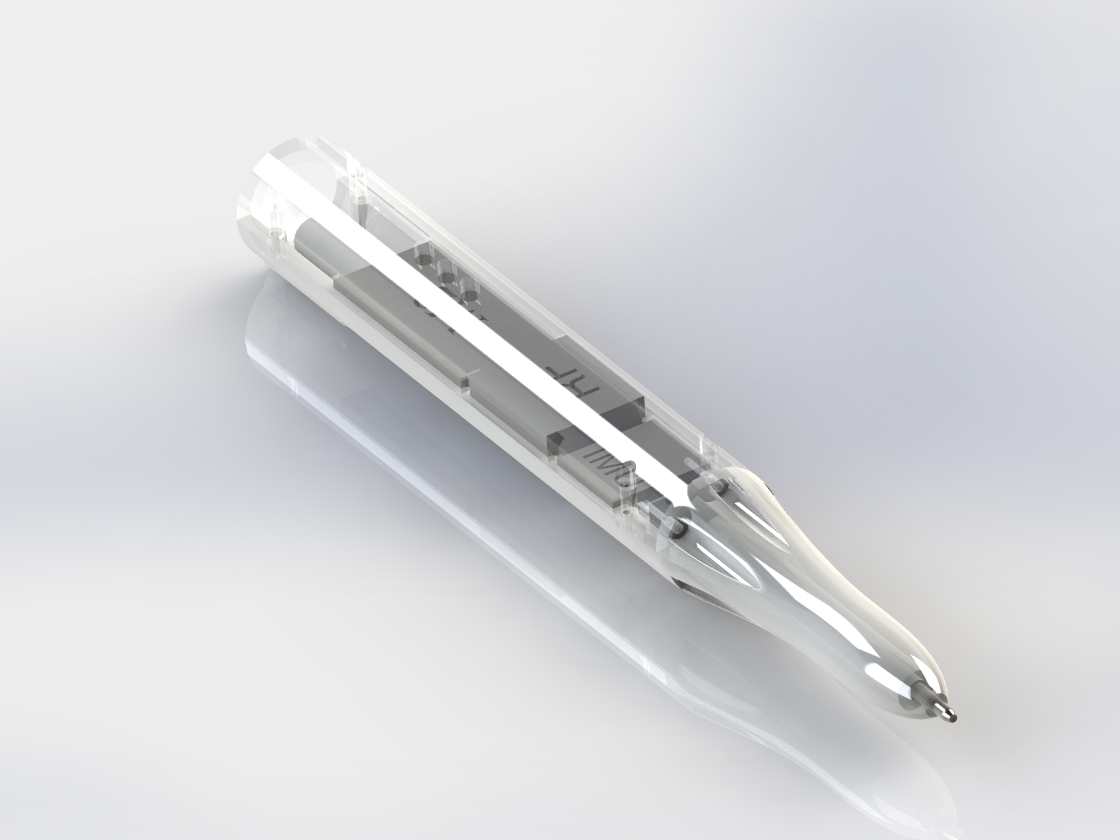
\includegraphics[width=0.5\textwidth, height= 5cm]{pen_render.png}
    \caption{Rendering of the 3D printed model of the penn}
\end{figure}

An ATMega32u4 microcontroller provides onboard processing and interfaces to the wireless module, IMU, switch, and indicator LEDs. Two Nordic nRF24LE1 transceivers handle wireless communication between the pen and base station computer. Inertial measurements are provided by an MPU6050 digital IMU with configurable gain triaxial accelerometers and gyroscopes. A Honeywell HMC5883L triaxial magnetometer provides a reference to earth's magnetic field for orientation. A contact switch behind the pen tip detects contact with the page for character segmentation. Three LEDs on the case display pen state. The pen also includes onboard batteries, power management, and an on-off switch.
In this project, we use accelerometer sensitivity of +/-2g (0.59 milimeter per second squared resolution) and gyro sensitivity of +/-250 degrees per second (7.6 milidegrees per second resolution) for high resolution across accelerations and speeds encountered in writing. 
%As you can see, we have an on-board microprocessor, 3 axis accelerometer, 3 axis gyroscope, magnetometer, and WiFi module. It also has a very sensitive switch that can tel us when the pen is actually writing. On top of that, the pen has 3 LED lights to make a visual recognition of the states the pen was at. We also included in the real version, a switch to turn it on and off, and batteries.

\section{Data Processing} 
Raw inertial measurements are pre-processed in in several stages to generate features used in our learning algorithm. Two features sets have been considered: raw time-domain acceleration signals and integrated character images. As character recognition was a component of the third CIS519 assignment, we opted to focus on the integrated character image in our work thus far. In this approach, the IMU measurements are used to estimate the accelerations of the pen tip across the page which are twice integrated to estimate the trajectory of the pen tip and corresponding appearance of the character on the page. This processing involves five steps detailed in the following sections: data aquisition and preparation, attitude estimation and gravity cancellation, coordinate transformation, and finally integration and image generation.

\subsection{Data aquisition and Preparation}
Measurements from the IMU and contact switch onboard the pen are streamed wirelessly to a computer for processing. The computer logs seven signals: triaxial acceleration, triaxial angular velocities, and contact switch state (depressed or released). Acceleration and angular velocity signals are scaled to engineering units (meters per second squared and radians per second respectively) for all following operations. Both acceleration and angular velocity signals are passed through first-order low pass filters to reduce high frequency noise introduced by the sliding of the pen tip across the page in writing.

\subsection{Attitude Estimation and Gravity Cancellation}
In order to integrate the tip accelerations, the measured acceleration due to gravity must be removed from the acceleration signals and the pen motions must be translated first to the pen tip and then into the plane of the page. All of these operations require knowledge of the pen's orientation relative to gravity. Pen attitude estimation is implemented using Sebastian Madgwick's open-source work. To counter gyro-integration drift in rotation about the vertical axis, the vertical axis rotation is high pass filtered. Using the pen attitude estimate, the acceleration and angular velocity vectors are rotated into the world frame with gravity along the z axis. Gravity can then be subtracted from the acceleration vector to obtain the acceleration of the pen relative to the page.

\subsection{Coordinate Transformation}
Accelerations and rotations of the pen body measured at the IMU are translated to the tip by the following transform:

\textbf{P}: location of the IMU \\
\textbf{O}: origin of frame G on the page \\
\textbf{frame G}: SRT fixed to the page with origin O (ground frame) \\
\textbf{frame M}: SRT fixed to the pen at the IMU with origin at point P (pen frame) \\
\textbf{Q}: location of the pen tip \\
$\underset{\mbox{\textasciitilde}}{\tmop{\textbf{PQ}}}$: vector from the IMU origin to
the pen tip

The acceleration of the pen tip in the ground frame is given by:
\begin{align*}
  ^G \underset{\mbox{\textasciitilde}}{a}^Q =^G
  \underset{\mbox{\textasciitilde}}{a}^P +^M
  \underset{\mbox{\textasciitilde}}{a}^Q &+^G
  \underset{\mbox{\textasciitilde}}{\alpha}^P \times
  \underset{\mbox{\textasciitilde}}{\tmop{PQ}} + 2^G
  \underset{\mbox{\textasciitilde}}{w}^M \times^M
  \underset{\mbox{\textasciitilde}}{v}^Q + ... \\ &+ ^G 
  \underset{\mbox{\textasciitilde}}{w}^M \times \left(^G
  \underset{\mbox{\textasciitilde}}{w}^M \times
  \underset{\mbox{\textasciitilde}}{\tmop{PQ}} \right)
\end{align*}
Since point Q (the pen tip) is fixed in frame M (the pen frame), $^M
\underset{\mbox{\textasciitilde}}{a}^Q$ and $^M
\underset{\mbox{\textasciitilde}}{v}^Q$ are both 0. The above equation simplifies to:
\begin{eqnarray*}
  & ^G \underset{\mbox{\textasciitilde}}{a}^Q =^G
  \underset{\mbox{\textasciitilde}}{a}^P +^G
  \underset{\mbox{\textasciitilde}}{\alpha}^P \times
  \underset{\mbox{\textasciitilde}}{\tmop{PQ}} +^G
  \underset{\mbox{\textasciitilde}}{w}^M \times \left(^G
  \underset{\mbox{\textasciitilde}}{w}^M \times
  \underset{\mbox{\textasciitilde}}{\tmop{PQ}} \right) & 
\end{eqnarray*}
The IMU measures accelerations and angular velocities of frame M relative to frame G expressed in frame M. \ Using the attitude estimate, these measurements can be rotated into frame G to produce $^G
\underset{\mbox{\textasciitilde}}{a}^P$ and $^G
\underset{\mbox{\textasciitilde}}{w}^M \nosymbol$. \ The angular acceleration
$^G \underset{\mbox{\textasciitilde}}{\alpha}^P$ is obtained by numerically
differentiating $^G \underset{\mbox{\textasciitilde}}{w}^M$.

\subsection{Integration and Image Generation}
The trajectory of the pen tip in the page frame is obtained by twice-integrating $^G \underset{\mbox{\textasciitilde}}{a}^Q$.
Since the velocity and position are integrations of noisy signals they are prone to very significant drift over time. To counteract this drift, the position and velocity estimates are re-zeroed at the start of every character and both the velocity and position are high pass filtered. The resulting trajectory can be plotted in the plane to approximate the appearance of the character on the page. This trajectory image is sampled to produce a black and white image which is then scaled and blurred to produce the final learning features.

% Data Streaming
%The first thing we had to do was to get raw data readings from the pen. After a couple of trials and for the sake of time saving, we decided that we would have a better first approach streaming the data out through USB instead of WiFi, to get a higher density of readings (WiFi is slower, saturates faster). Though the pen still has the functionality and all the programming to send the data via WiFi, we are more interested in getting the data out as soon as possible. Once that was done, we could pass to the next big task, data pre-processing.
% Filtering the data
%The raw data you get out of this readings is really noisy. It cannot be used in any way like it is. The data needs to be filtered to get the attitude estimation. We use a Kalman Filter to get the attitude estimation, which will give us the orientation of the pen relative to gravity and the page (Which has to be on a flat surface, and cannot be moving).
%We use this to subtract the gravity components in the vectors that they are appearing, so in this way we prevent drifting on those readings. We also get out of this the rotation of the pen relative to the page, which we will then use for further filtering.
% More filtering... and trajectory tracking
%Once we have the pre-filtered data, we can get a cleaner reading of the acceleration of the tip of the pen (relative to the page), which we will use to get a trajectory estimation. We integrate the acceleration twice, while at the same time, high-pass filtering any long time drifting of the readings in both yaw angle and velocities.
%Differentiation of $^G \underset{\mbox{\textasciitilde}}{w}^M$ greatly increases high-frequency noise in the acceleration estimate which must be low-pass filtered. More problematic, double-integration of the acceleration estimate compounds small steady errors which build up to large velocity errors and even larger position errors. This necessitates high-pass filtering of both the velocity and position signals. These high-pass filters are ineffective both at removing low-frequency drift and maintaining good signal quality resulting in unusably noisy and drift-filled position estimates.

\subsection{Preliminary Results}
The integrated character image is prone to distortion due to velocity and position drift over the course of writing the character. Our current filtering schemes are somewhat successful at reducing integration drift and rejecting noise from vibration, but character distortion is still significant. An example character integration is shown below.
%After some trials and errors, we finally de-bugged the code to get some character images that we could then use with the neural nets that we have already implemented on class, to get some character recognition via class classification.
%The results from all the estimations give us characters like the one below.
\begin{figure}[H]
\centering
    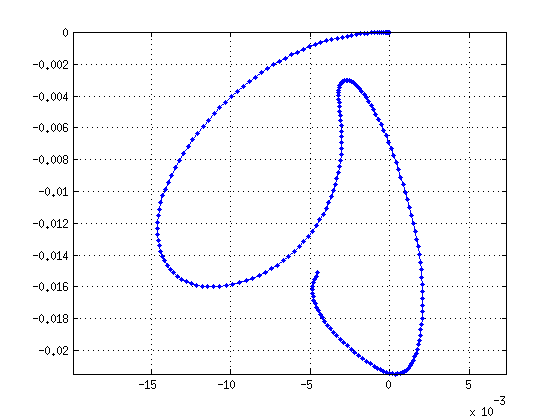
\includegraphics[width=0.5\textwidth, height= 5cm]{g.png}
    \caption{Processed written letter "g"}
\end{figure}


\subsection{Next Steps}
After some thinking on the results we are getting and the complexity of the math behind all this, we are presented with two different options. Keep on pushing for this approach to get all the character representations in an image base, or shifting our Machine Learning algorithm to Hidden Markov Models which would potentially require a lot less data pre-processing and a more complicated machine learning implementation.
 
\section*{Acknowledgments} 
 
Attitude estimation Kalman Filter and initial approximation provided by \textbf{open-source} code from Sebastian Madgwick (July 2012), based on his paper \textbf{Estimation of IMU and MARG orientation using a gradient descent algorithm}.\\
For trajectory reconstruction, consulted Jeen-Shing Wang, Yu-Liang Hsu, and Jiun-Nan Liu's paper entitled \textbf{An Inertial-Measurement-Unit-Based Pen With a Trajectory Reconstruction Algorithm and Its Applications}.
\bibliography{example_paper}
\bibliographystyle{icml2014}

\end{document} 


% This document was modified from the file originally made available by
% Pat Langley and Andrea Danyluk for ICML-2K. This version was
% created by Lise Getoor and Tobias Scheffer, it was slightly modified  
% from the 2010 version by Thorsten Joachims & Johannes Fuernkranz, 
% slightly modified from the 2009 version by Kiri Wagstaff and 
% Sam Roweis's 2008 version, which is slightly modified from 
% Prasad Tadepalli's 2007 version which is a lightly 
% changed version of the previous year's version by Andrew Moore, 
% which was in turn edited from those of Kristian Kersting and 
% Codrina Lauth. Alex Smola contributed to the algorithmic style files.  
